Nous ajoutons maintenant du bruit blanc gaussien au signal modulé.
Rappelons qu'un bruit blanc est un bruit de moyenne nulle et un bruit gaussien est un bruit distribué selon une loi normale.
Pour cela, nous ajoutons une pertubation de puissance déduite $P_b$ en fonction du rapport signal sur bruit ${SRN_db}$ que nous voulons : \[P_b=\frac{P_x}{10^{\frac{SNR_{dB}}{10}}}\]
Nous calculons d'abord la puissance $P_x$ du signal $x(t)$ (ligne 1), puis la puissance $P_b$ (ligne 3). Nous ajoutons enfin le bruit au signal $x(t)$ (ligne 4).
\begin{lstlisting}[caption=Ajout de bruit blanc gaussien]
Px = mean(abs(x).^2);         % puissance du signal
SNRdb = 50;                   % rapport signal sur bruit
Pb = Px / (10^(SNRdb / 10));  % puissance du bruit
x = x + Pb * randn(1, Ns * Nb_bit);
\end{lstlisting}
\begin{figure}[ht!]
   \centering
   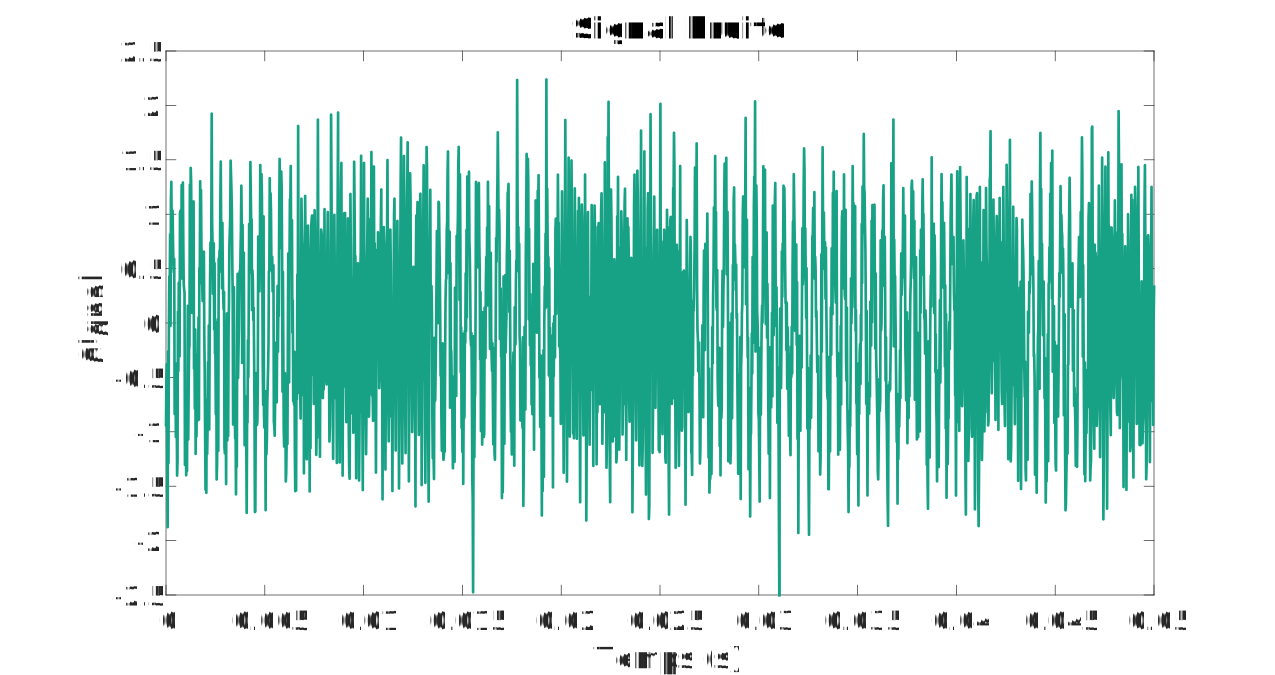
\includegraphics[scale=0.4]{partie-2/sous-partie-2/2.2.1.png}
   \caption{Signal bruité \label{fig : buit}}
\end{figure}
La Figure \ref{fig : buit} représente le signal bruité. La modulation en fréquence est bien visible.